% this chapter is basically covered by
% - Optimizations https://cds.cern.ch/record/2912217
% - Acts integration https://cds.cern.ch/record/2921878
% - Expected tracking performance https://arxiv.org/abs/2412.15090
% - TDR https://cds.cern.ch/record/2802799

The new inner tracking detector (ITk) for the ATLAS experiment is designed to cope with the high luminosity and pileup conditions expected in the High-Luminosity Large Hadron Collider (HL-LHC) era. The ITk is a full-silicon detector and will be composed of a pixel \cite{itk-pixel-tdr} and strip \cite{itk-strip-tdr} subsystem. This upgrade is not only challening for the detector design, construction, and opteration, but also the track reconstruction software. The ATLAS collaboration is corrently working on upgrading the reconstruction software for Run-4, which is the first run with the new detector. This includes migrating to the Acts toolkit for track reconstruction, for both the inner detector and the muon spectrometer. Part of the work on this thesis was to integrate the Acts track finding algorithm into the ATLAS track reconstruction software, which was a joint effort and performed in close collaboration with the Acts-ITk team.

Apart from the software upgrade, the ATLAS collaboration is currently working on a new trigger system for Run-4 and evaluates different hardware technologies to realize the high-level trigger (HLT). The Acts-based track reconstruction chain is one of the candidates, as a CPU-based solution. Other candidates are GPU-based and FPGA-based.

\section{Acts-based track reconstruction chain}

The Acts-based track reconstruction chain was planned to use the same reconstruction steps as the existing reconstruction chain, referred to as the \textit{legacy chain}. The legacy chain is based on Run-3 reconstruction and tuned to some degree for Run-4. The motivation for the Acts-based chain is increase maintainability and potentially performance. The ATLAS track reconsturction software was written in the early 2000s and its authors are no longer available. New people entering the collaboration are faced with a large amount of legacy code which is poorly documented and difficult to understand. For this reason, the ATLAS collaboration decided to adopt the Acts toolkit for the Run-4 track reconstruction, as it promises to be modern, maintainable, documented, and efficient from the start.

For this purpose, some reconstruction algorithms have been ported from legacy to Acts and validated against the legacy chain. An example for this is the triplet seeding algorithm. Other algorithms, like the Kalman-based track finding and fitting, have been implemented from scratch in Acts, based on literature and experience from the legacy chain. One of the main benefits of Acts is its experiment-agnostic design, which allows to use the same code for different experiments. Other experiments can benefit from existing, validated reconstruction code, and potentially contribute to the development of the Acts toolkit. ATLAS will then also benefit from the experience of other experiments, and the code can be shared between different experiments.

The Acts-based track reconstruction chain can be used for offline reconstruction, as well as for the HLT. The HLT is part of the ATLAS trigger system and makes the final decision on whether an event is stored on disk or fully discarded. The ATLAS collaboration is currently working on a new trigger system for Run-4 and evaluates different hardware technologies to realize the HLT. The Acts-based track reconstruction chain is one of the candidates, as a CPU-based solution. Other candidates are GPU-based and FPGA-based.

The legacy and Acts-based reconstruction chain are very close to what was described in the introduction in Section \ref{sec:intro/reco/reco-steps}. The main pass, which reconstructs tracks from the primary interactions, starts from raw sensor data. The raw data is clustered and measurements are formed. The measurements are used to form spacepoints, which are the input for the seeding algorithm. The seeding algorithm finds potential starting points for tracks, which are used by the track finding algorithm to find tracks. The clusterization, spacepoint formation, and seeding steps are performed separately for pixels and stips. The track finding step combines pixel and stip seeds to form a single track collection.

One main difference between the legacy and Acts-based chain is the track finding algorithm. While the legacy chain focuses only on finding compatible measurements, the Acts-based chain deploys a fully-fledged Kalman filter to not only find but also fit tracks simultaneously. Due to this, the Acts-based chain does not need a separate fitting step, which is required in the legacy chain.

Apart from that, the Acts-based chain only deploys a simplistic ambiguity resolution algorithm for now, which is based on the greedy approach described in Section \ref{sec:dev/general/greedy-ambiguity-resolution}. The legacy chain uses a more sophisticated ambiguity resolution algorithm, which is also able to resolve cluster ambiguities and refit tracks based on this information. How this will be implemented in the Acts-based chain is currently under investigation.

\section{CPU performance optimizations}

Since compute resources will be limited for reconstructing the large amount of data expected from the HL-LHC, the Acts-based chain does not only need to deliver similar physics performance as the legacy chain, but perform at least as good as the legacy chain in terms of CPU time. To achieve this, the Acts-based chain has been optimized over several iterations. This was carried out by the Acts-ITk team and as part of the work on this thesis. Some of these optimizations have already been described in Chapter \ref{ch:dev/track_finding}.

\begin{figure}[h]
    \centering
    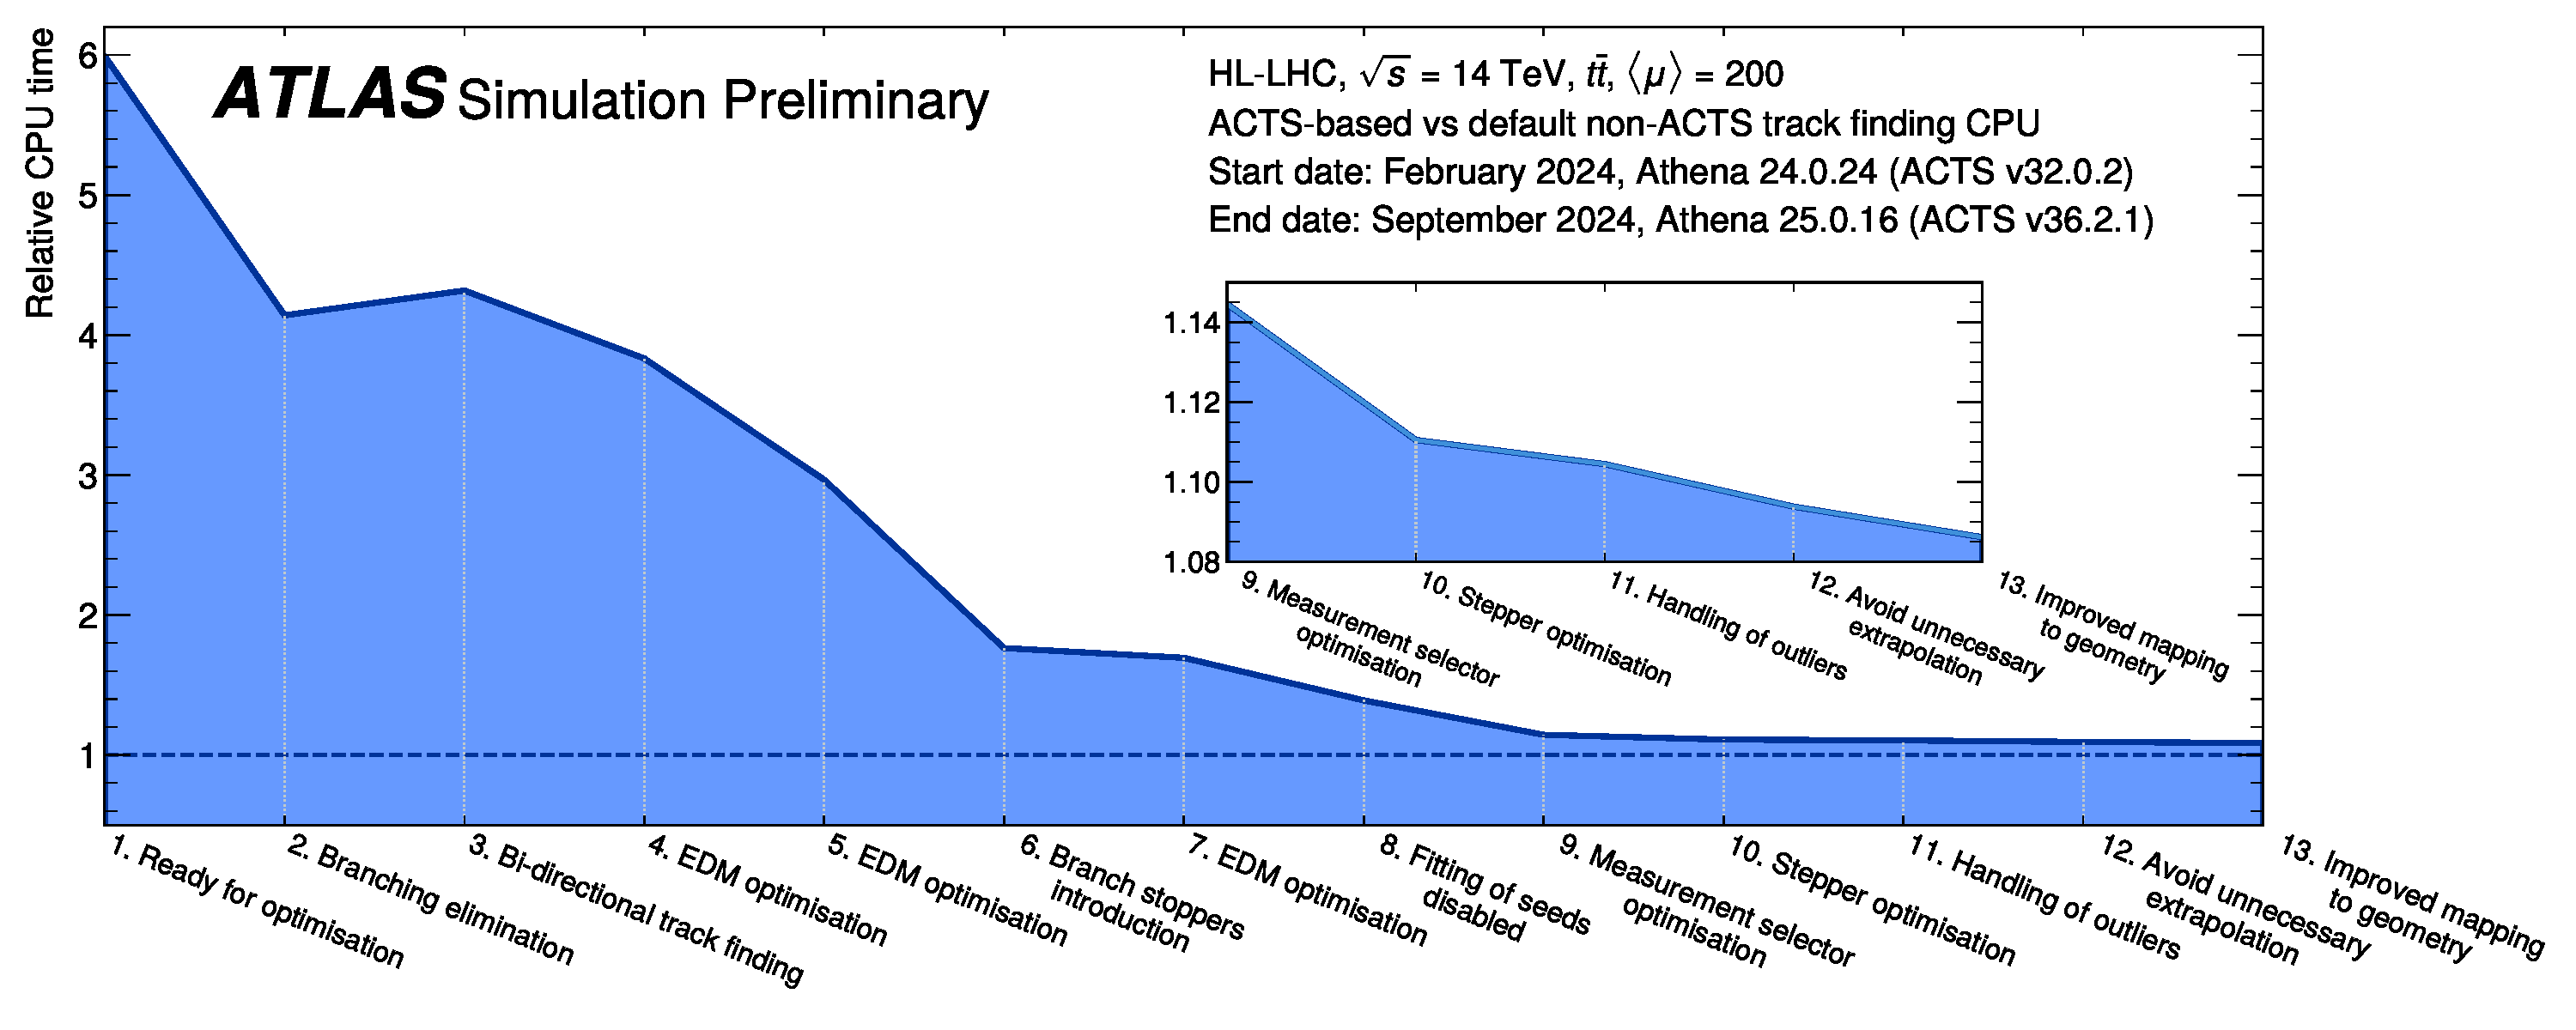
\includegraphics[width=1.15\textwidth]{parts/3_performance/12_athena-performance/figures/cpu_improvements.pdf}
    \caption{Incremental improvements to the compute time for reconstructing \ttbar events at $\langle \mu \rangle$ = 200 with the ATLAS reconstruction software Athena \cite{pubnote-2024-017}. The CPU time shown only accounts for track finding, and it is relative to the legacy counterpart. A zoomed version of the last 5 data points is also shown.}
    \label{fig:perf/itk/cpu-improvements}
\end{figure}

Figure \ref{fig:perf/itk/cpu-improvements} shows the incremental improvements to the compute time for reconstructing \ttbar events at $\langle \mu \rangle$ = 200 with the ATLAS reconstruction software Athena \cite{pubnote-2024-017}. The starting date for the plot is 15 February 2024, using Athena 24.0.24 (ACTS v32.0.2). The relevant improvements are reported in chronological order on the horizontal axis of the plot and are described in the text. The last data point on the plot corresponds to the running time obtained on 10 September 2024 using Athena 25.0.16 (ACTS v36.2.1).

The individual improvements shown in Figure \ref{fig:perf/itk/cpu-improvements} are:
\begin{enumerate}
    \item \textbf{Ready for optimization}: the starting point for the optimizations, corresponding to the first  fullyfunctional version of the ACTS-based ITk track reconstruction deployed in Athena 24.0.24 (ACTS v32.0.2) on 15 February 2024. This version of the code was measured to be six times slower than the legacy ITk track finding.
    \item \textbf{Branching elimination}: the combinatorial Kalman filter is configured to only consider a single branch. Hence proving one input seed can at most result in a single track candidate. The justification for this is that the triplet seeding algorithm already explores the measurement combinatorics and the track finding does not need to do this again.
    \item \textbf{Bi-directional track finding}: enabling track finding to search for measurements both outward(i.e. away from the interaction point) and inward. This is described in more detail in Section \ref{sec:dev/trackfinding/two-way}.
    \item \textbf{EDM optimization}: improved storage and access of the seed containers.
    \item \textbf{EDM optimization}: better usage of internal representation of track containers.
    \item \textbf{Branch stoppers introduction}: usage of early branch-aborting conditions to stop the track finding and decide whether to keep the track candidate.
    \item \textbf{EDM optimization}: simplification of measurement access from track states. These developments lead to a more general improvement of measurement projection in Acts described in Section \ref{sec:dev/general/measurement-projection}.
    \item \textbf{Fitting of seeds disabled}: avoiding seed parameter refinement using a Kalman filter. This was shown not to be critical for the track finding performance, especially in the pixels.
    \item \textbf{Measurement selector optimization}: improved selection and calibration of measurements during track state creation for the combinatorial Kalman filter.
    \item \textbf{Stepper optimizations}: faster implementation of the numerical integration and the Jacobian and covariance transport. This is described in more detail in Section \ref{sec:dev/stepper/sympy}.
    \item \textbf{Handling of outliers}: implementation of a dedicated outlier compatibility criterion. Define a maximum number of outliers allowed per track and stop track finding earlier if the limit is exceeded.
    \item \textbf{Avoid unnecessary extrapolation}: avoiding unnecessary extrapolation at the end of track finding, in case this is already performed by the inward extension.
    \item \textbf{Improved mapping to geometry}: improved mapping of detector elements and measurements to tracking geometry surfaces.
\end{enumerate}

At the end of the optimizations, the Acts-based track finding was measured to be about 8\% slower than the legacy track finding. This is a significant improvement compared to the starting point. Given the fact that the Acts-based chain does not need a separate fitting step, the overall performance of the Acts-based chain is expected to be better than the legacy chain. However, not all algorithms have been ported to Acts yet, including a more sophisticated ambiguity resolution algorithm that deals with cluster ambiguities. Only after the chains are feature equivalent, a fair comparison can be made. This is an ongoing effort.

Given the current workload of the track finding algorithm, it appears that its CPU performance cannot be significantly improved further. A potential bottleneck is the triplet seeding algorithm, which produces a large number of fake seeds, which need then to be filtered out be the track finding algorithm. This is currently under investigation. Other seeding algorithms exist, which produce less fakes and show promising CPU performance \cite{acts-gbts}. However, these algorithms are not yet fully available in Acts. The Acts-ITk team is currently working on integrating these algorithms into Acts and the Acts-based ITk chain.

\section{Physics performance}

\begin{itemize}
    \color{red}
    \item only if we are brave
    \item single particle efficiency, fake rate, duplication rate, resolution, pulls
    \item ttbar efficiency, fake rate, duplication rate, pileup dependence
\end{itemize}

\section{Summary, conclusion and outlook}

\begin{itemize}
    \color{red}
    \item a lot of progress has been made
    \item acts based chain is very close to legacy chain
    \item seeding seems to be the main cpu bottleneck due to high fake rate
    \item what is missing?
    \begin{itemize}
        \item single muon efficiency
        \item electron reconstruction
    \end{itemize}
    \item material map might need optimization
\end{itemize}
